\PassOptionsToPackage{unicode=true}{hyperref} % options for packages loaded elsewhere
\PassOptionsToPackage{hyphens}{url}
\documentclass[11pt,dvipsnames,ignorenonframetext,aspectratio=169]{beamer}
\IfFileExists{pgfpages.sty}{\usepackage{pgfpages}}{}
\setbeamertemplate{caption}[numbered]
\setbeamertemplate{caption label separator}{: }
\setbeamercolor{caption name}{fg=normal text.fg}
\beamertemplatenavigationsymbolsempty
\usepackage{lmodern}
\usepackage{amssymb,amsmath}
\usepackage{ifxetex,ifluatex}
\usepackage{fixltx2e} % provides \textsubscript
\ifnum 0\ifxetex 1\fi\ifluatex 1\fi=0 % if pdftex
  \usepackage[T1]{fontenc}
  \usepackage[utf8]{inputenc}
\else % if luatex or xelatex
  \ifxetex
    \usepackage{mathspec}
  \else
    \usepackage{fontspec}
\fi
\defaultfontfeatures{Ligatures=TeX,Scale=MatchLowercase}







\fi

  \usetheme[]{monash}

  \usecolortheme{monashwhite}


% A default size of 24 is set in beamerthememonash.sty
  \setbeamerfont{title}{series=\bfseries,parent=structure,size=\fontsize{20pt}{32}}

% Title page
\setbeamertemplate{title page}
{\placefig{-0.01}{-0.01}{width=1.01\paperwidth,height=1.01\paperheight}{genetic\_variation\_awn\_barley.png}
\begin{textblock}{7.5}(1,2.8)\usebeamerfont{title}
{\color{blue}\raggedright\par\inserttitle}
\end{textblock}
\begin{textblock}{7.5}(1,7)
{\color{blue}\raggedright{\insertauthor}\mbox{}\\[0.2cm]
\insertdate}
\end{textblock}}


  \useinnertheme{rounded}

  \useoutertheme{smoothtree}

% use upquote if available, for straight quotes in verbatim environments
\IfFileExists{upquote.sty}{\usepackage{upquote}}{}
% use microtype if available
\IfFileExists{microtype.sty}{%
  \usepackage{microtype}
  \UseMicrotypeSet[protrusion]{basicmath} % disable protrusion for tt fonts
}{}


\newif\ifbibliography
  \usepackage[round]{natbib}
  \bibliographystyle{plainnat}


\hypersetup{
      pdftitle={Introduction to Resistance Breeding},
            colorlinks=true,
    linkcolor=red,
    citecolor=Blue,
    urlcolor=lightgrayd,
    breaklinks=true}
%\urlstyle{same}  % Use monospace font for urls







% Prevent slide breaks in the middle of a paragraph:
\widowpenalties 1 10000
\raggedbottom

  \AtBeginPart{
    \let\insertpartnumber\relax
    \let\partname\relax
    \frame{\partpage}
  }
  \AtBeginSection{
    \ifbibliography
    \else
      \let\insertsectionnumber\relax
      \let\sectionname\relax
      \frame{\sectionpage}
    \fi
  }
  \AtBeginSubsection{
    \let\insertsubsectionnumber\relax
    \let\subsectionname\relax
    \frame{\subsectionpage}
  }



\setlength{\parindent}{0pt}
\setlength{\parskip}{6pt plus 2pt minus 1pt}
\setlength{\emergencystretch}{3em}  % prevent overfull lines
\providecommand{\tightlist}{%
  \setlength{\itemsep}{0pt}\setlength{\parskip}{0pt}}

  \setcounter{secnumdepth}{0}


%% Monash overrides
\AtBeginSection[]{
   \frame<beamer>{
   \frametitle{Outline}\vspace*{0.2cm}
   
   \tableofcontents[currentsection,hideallsubsections]
  }}

% Redefine shaded environment if it exists (to ensure text is black)
\ifcsname Shaded\endcsname
  \definecolor{shadecolor}{RGB}{225,225,225}
  \renewenvironment{Shaded}{\color{black}\begin{snugshade}\color{black}}{\end{snugshade}}
\fi
%%


  \usepackage{setspace}
  \usepackage{wasysym}
  % \usepackage{footnote} % don't use this this breaks all
  \usepackage{fontenc}
  \usepackage{fontawesome}
  \usepackage{booktabs,siunitx}
  \usepackage{longtable}
  \usepackage{array}
  \usepackage{multirow}
  \usepackage{wrapfig}
  \usepackage{float}
  \usepackage{colortbl}
  \usepackage{pdflscape}
  \usepackage{tabu}
  \usepackage{threeparttable}
  \usepackage{threeparttablex}
  \usepackage[normalem]{ulem}
  \usepackage{makecell}
  \usepackage{xcolor}
  \usepackage{tikz} % required for image opacity change
  \usepackage[absolute,overlay]{textpos} % for text formatting
  \usepackage{chemfig}
  \usepackage[skip=0.333\baselineskip]{caption}
  % \newcommand*{\AlignChar}[1]{\makebox[1ex][c]{\ensuremath{\scriptstyle#1}}}%
  \usepackage{siunitx}

  % this font option is amenable for beamer
  \setbeamerfont{caption}{size=\tiny}
  \singlespacing
  \definecolor{lightgrayd}{gray}{0.95}
  \definecolor{skyblued}{rgb}{0.65, 0.6, 0.94}
  \definecolor{oranged}{RGB}{245, 145, 200}

  % % better to insert it into template itself
  % \newlength{\cslhangindent}
  % \setlength{\cslhangindent}{1.5em}
  % \newenvironment{cslreferences}%
  %   {\setlength{\parindent}{0pt}%
  %   \everypar{\setlength{\hangindent}{\cslhangindent}}\ignorespaces}%
  %   {\par}

  \usepackage[caption=false]{subfig}

  \newcommand{\bcolumns}{\begin{columns}[T, onlytextwidth]}
  \newcommand{\ecolumns}{\end{columns}}

  \newcommand{\bdescription}{\begin{description}}
  \newcommand{\edescription}{\end{description}}

  \newcommand{\bitemize}{\begin{itemize}}
  \newcommand{\eitemize}{\end{itemize}}
  \AtBeginSubsection{}
  \captionsetup{skip=0pt,font=tiny,belowskip=-2pt,aboveskip=0pt}

  \title[]{Introduction to Resistance Breeding}


  \author[
        \vspace{-0.5cm}Deependra Dhakal\\
Agriculture and Forestry University\\
\textit{ddhakal.rookie@gmail.com}\\
\url{https://rookie.rbind.io}
    ]{\vspace{-0.5cm}Deependra Dhakal\\
Agriculture and Forestry University\\
\textit{ddhakal.rookie@gmail.com}\\
\url{https://rookie.rbind.io}}


\date[
      
  ]{
    }

\begin{document}

% Hide progress bar and footline on titlepage
  \begin{frame}[plain]
  \titlepage
  \end{frame}


   \frame<beamer>{
   \frametitle{Outline}\vspace*{0.2cm}
   
   \tableofcontents[hideallsubsections]
  }

\hypertarget{potential-yield}{%
\section{Potential Yield}\label{potential-yield}}

\begin{frame}{}
\protect\hypertarget{section}{}
\small

\begin{itemize}
\tightlist
\item
  Biological efficiency of production (expressed as unit of the product
  per unit of absorbed solar energy, or conveniently as kg/hectare) is a
  relative measurement and it varies according to the environment, with
  the cultivar, and especially with its variations.
\item
  A proper biological index could help plant breeders in obtaining
  cultivars with better efficiency in using natural resources.
\item
  Yield potential (a theoretical idea) can be defined as the yield
  obtained when the cultivar is grown with no environmental restrictions
  -- with no biotic or abiotic stresses.

  \begin{itemize}
  \tightlist
  \item
    soil nutrients and water are not limiting
  \item
    pests and weeds are effectively controlled
  \end{itemize}
\item
  Crop yield potential (genetic) is much larger than the biological
  efficiency per area (recorded yield) owing to several environmental
  influences and management practices -- collectively called
  \alert{stresses}.
\item
  Infection or infestation by plant pests and diseases affects
  \alert{yield} and \alert{end-use quality}
\end{itemize}
\end{frame}

\begin{frame}{}
\protect\hypertarget{section-1}{}
\begin{figure}
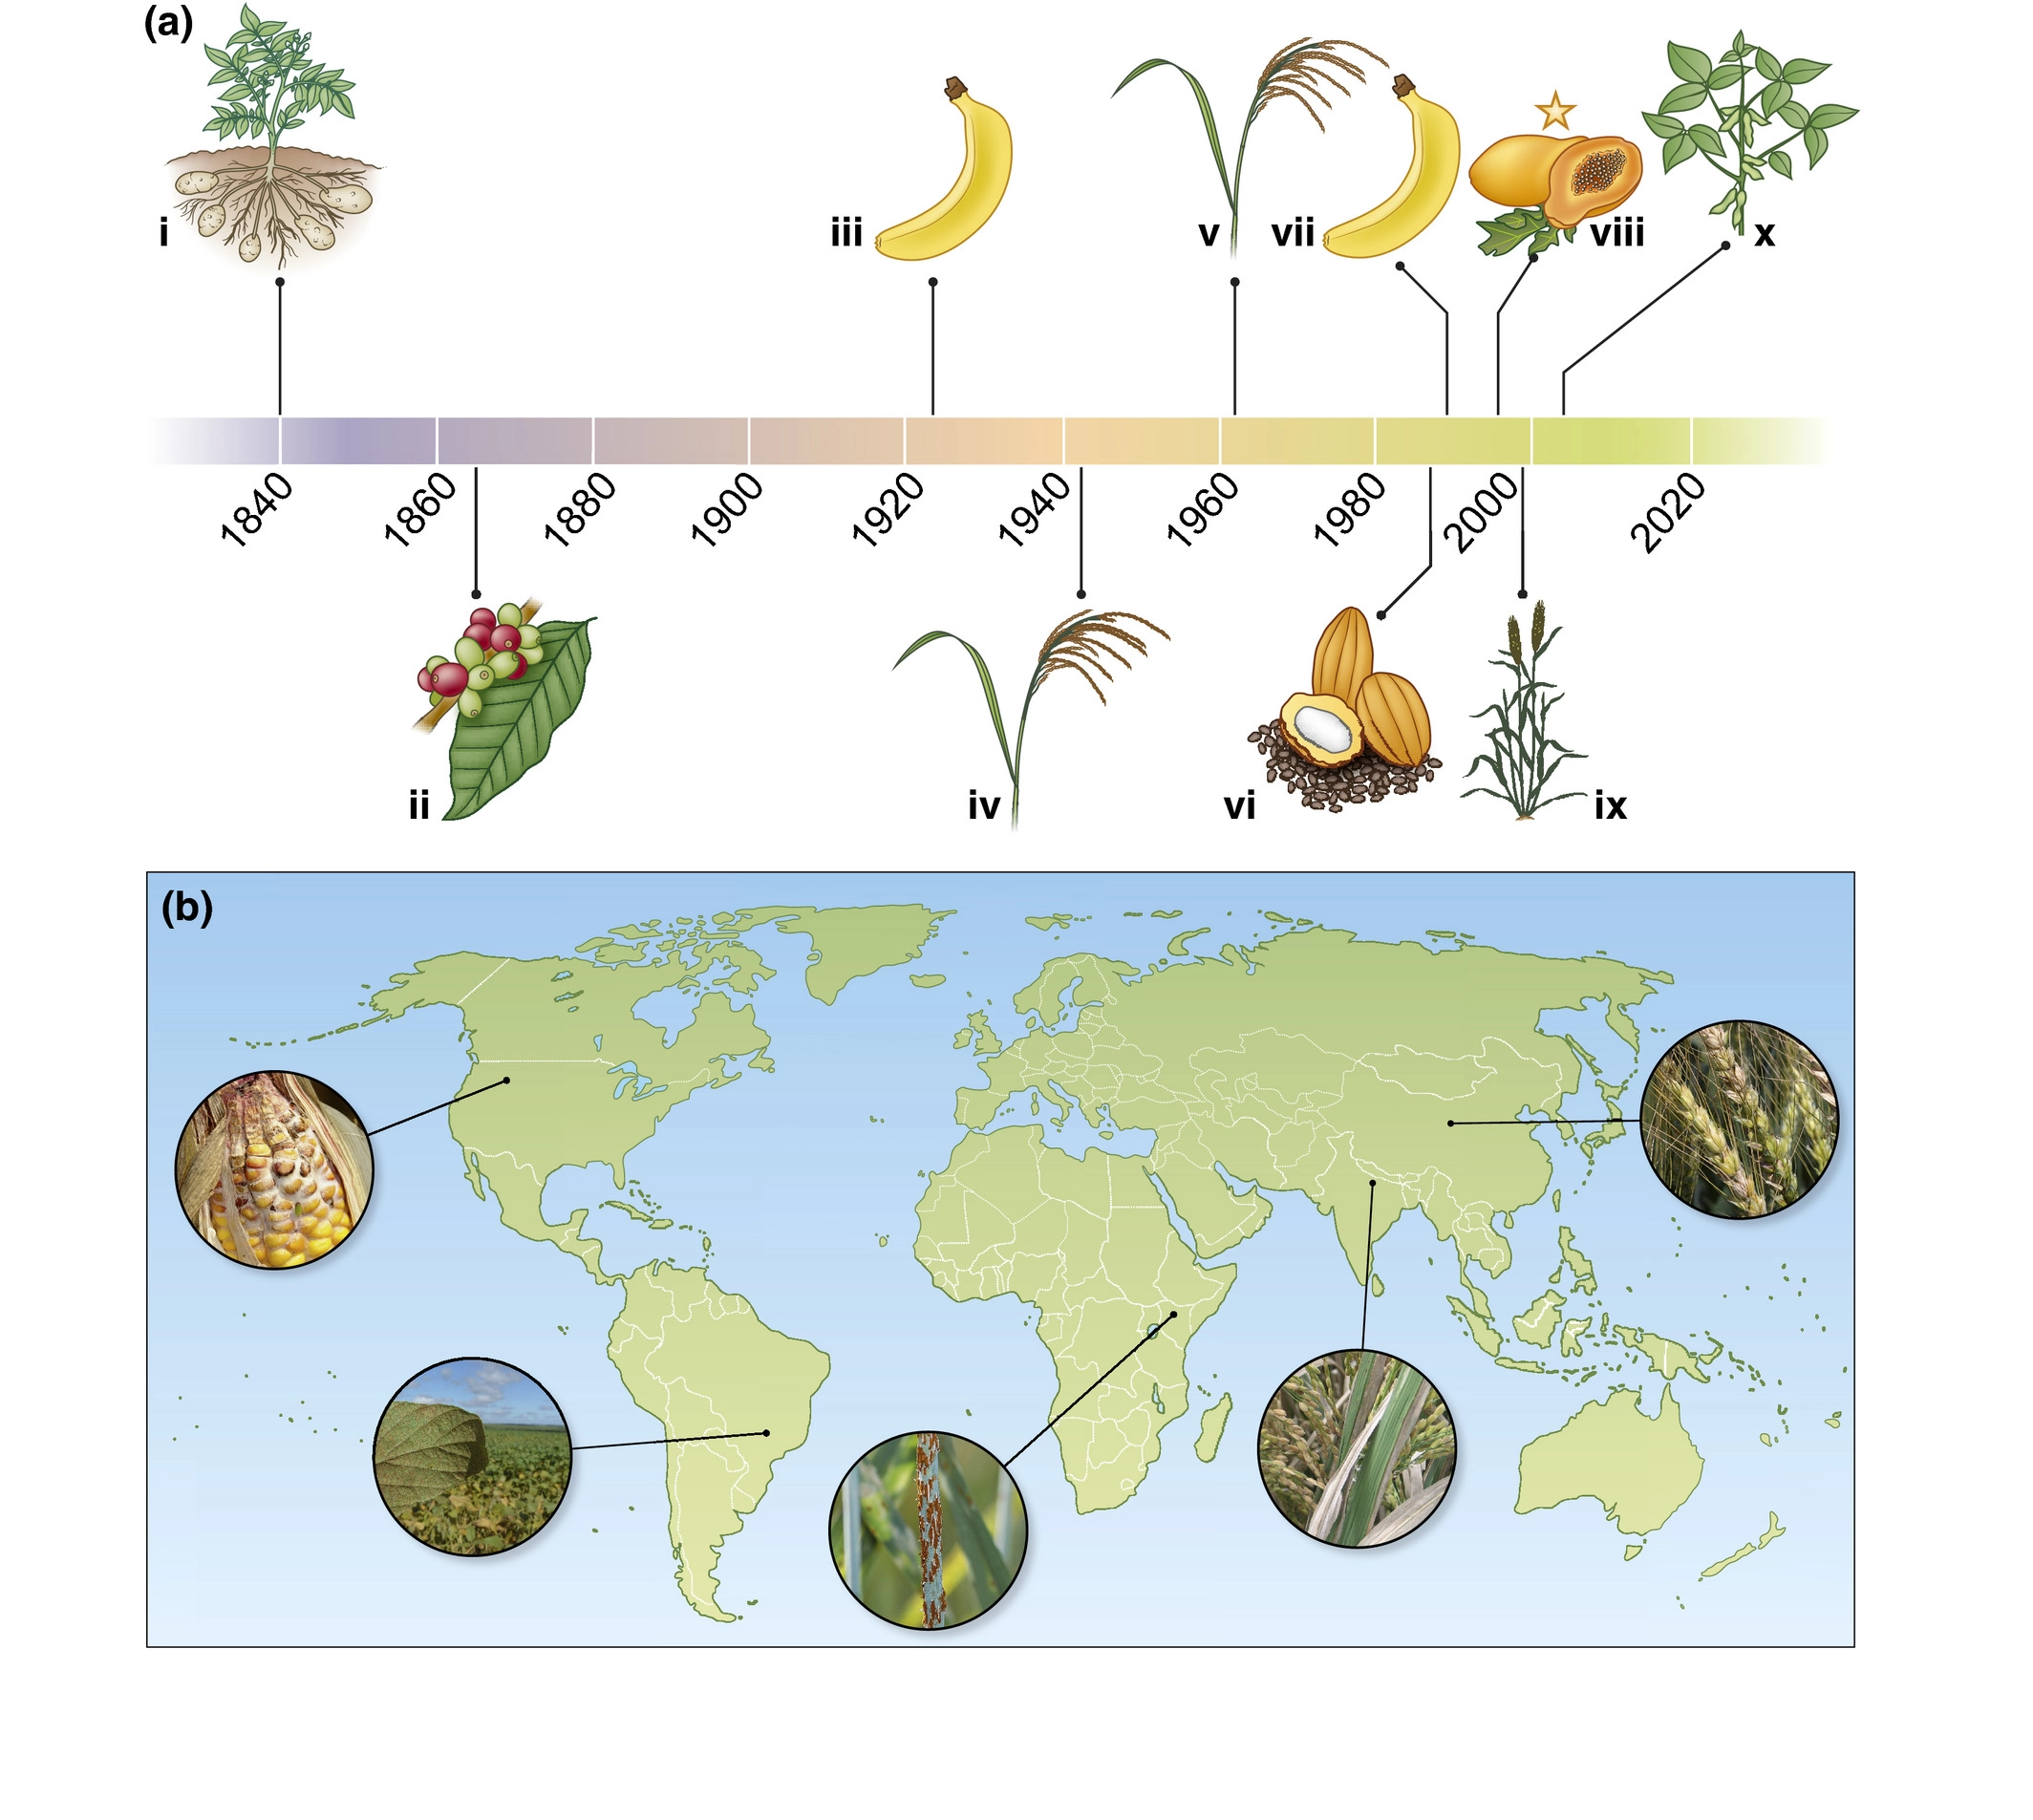
\includegraphics[width=0.4\linewidth]{../images/crop_pandemic_history} \caption{Major disease outbreaks in the last 150 years and current critical disease challenges. (i) Introduction of the oomycete \textit{Phytophthora infestans} which causes potato late blight. (ii) The rust fungus \textit{Hemileia vastatrix} wipes out the coffee crop in Sri-Lanka; the British become tea drinkers. (iii) The vascular fungal pathogen causing Fusarium wilt of banana nearly wipes out the Gros Michel variety; the resistant Cavendish banana is adopted. (iv) The fungus \textit{Cochliobolus miyabeanus}, which causes Brown spot disease of rice is a factor in the Great Bengal Famine in which 2 million people died of starvation. (v) Bacterial leaf blight or rice (\textit{Xanthomonas oryzae} pv. \textit{oryzae}) causes epidemics throughout Southeast Asia with yield losses up to 80\%. (vi) Witches' broom caused by the fungus \textit{Moniliophthora perniciosa} caused losses of upto 75\% of annual cacao production in Brazil. (vii) The new \textit{Fusarium} wilt isolate TR4 is identified and threatens Cavendish banana. (viii) Ringspot virus devastates the papaya industry in Hawaii; a GM variety is introduced that resists infection. (ix) A new race of the stem rust fungus \textit{Puccinia graminis} (UG99) is spreading throughout Africa and Middle East, threatening the world supply of wheat. (x) Asian soybean rust caused by \textit{Phakopsora pachyrhizi} reaches Brazil, costing growers US \$2 billion annually in damages and control measures.}\label{fig:crop-pandemic-history}
\end{figure}
\end{frame}

\begin{frame}{}
\protect\hypertarget{section-2}{}
\begin{figure}
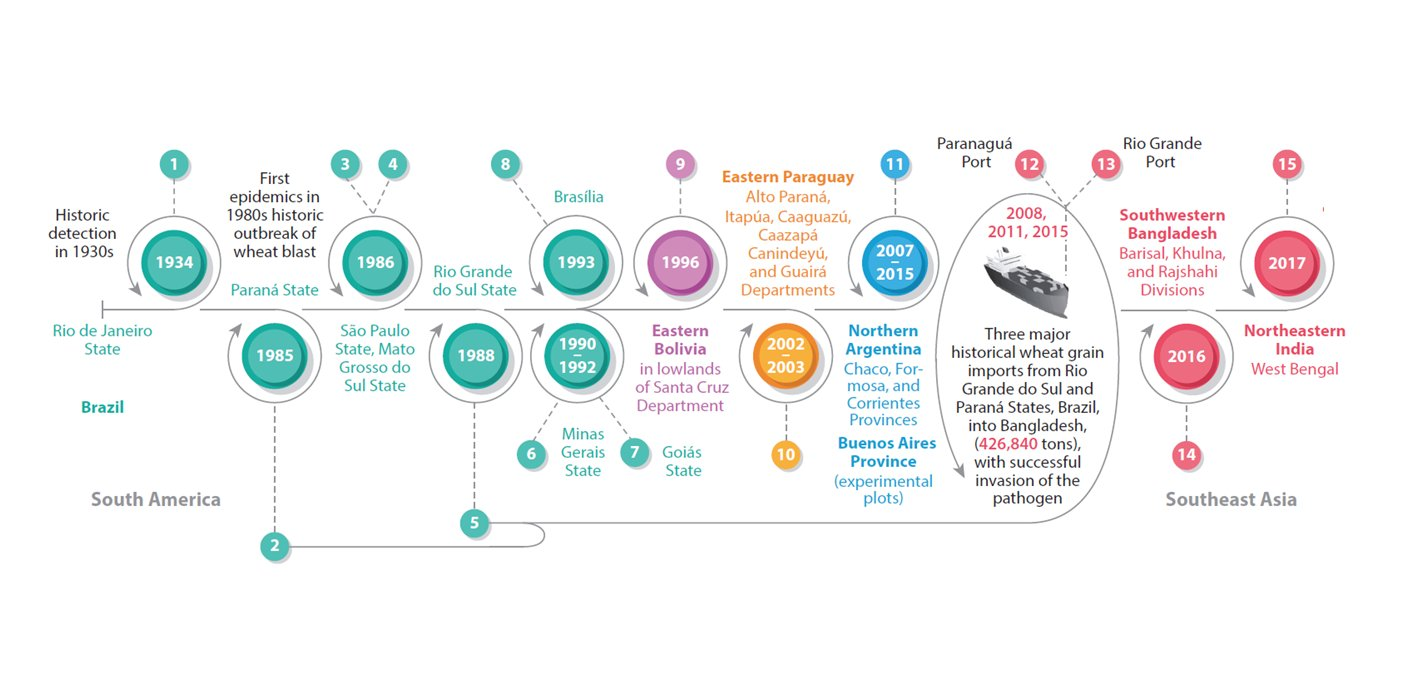
\includegraphics[width=0.86\linewidth]{../images/wheat_blast_distribution_due_brazil} \caption{Past present and future of Wheat blast. Countries that imported wheat from Brazil in 2016/17 are thought to have received much of the pathogen inoculums.}\label{fig:wheat-blast}
\end{figure}

\footnotesize Note: For more discussion on Wheat blast refer to
\citet{ceresini2018wheat}.
\end{frame}

\begin{frame}{}
\protect\hypertarget{section-3}{}
\begin{itemize}
\tightlist
\item
  Development of resistant cultivars involves consideration of the
  genetic variability of the pest/diseases as well as the variability in
  resistance (or sometimes tolerance) within the crop species or related
  group.
\item
  Durability of resistance is affected by emergence of new races of the
  disease/pest that are able to overcome existing resistance
\item
  Environmental changes (brought about by global warming) also affects
  the dynamics of plant interactions with pests and diseases and render
  crops more or less susceptible to biotic stresses, owing to:

  \begin{itemize}
  \tightlist
  \item
    changed distribution of phytophagous insects (lepidopterans)
  \item
    changes in crop and insect phenology synchrony (emergence)
  \item
    over one-third of the total variance in caterpillar parasitism
    (activity of natural predators) is explained by variability in
    precipitation
  \end{itemize}
\end{itemize}
\end{frame}

\begin{frame}{}
\protect\hypertarget{section-4}{}
\small

\begin{itemize}
\tightlist
\item
  Sources of alleles conferring disease resistance have traditionally
  been landraces and old cultivars/materials kept by small farmers.
\item
  A range of pests -- ranging upto large foraging mammals -- inflict
  crop damage, not all of which amenable to resistance breeding

  \begin{itemize}
  \tightlist
  \item
    Wheat crop in and around the wildlife protection buffer zones
    knocked down by a herd of Rhinoceri is hard! to breed for.\\
  \end{itemize}
\item
  For much of 20th century, scientific plant breeding has been
  successful in first 3 of 4 main objectives:

  \begin{itemize}
  \tightlist
  \item
    yield improvement
  \item
    quality improvement
  \item
    agronomic suitability improvement
  \item
    resistance to parasites
  \end{itemize}
\item
  \(\because\) resistance keeps breaking down because of new strains of
  the parasite and then an endless repetition of resistance failures and
  a ``boom and bust'' cycle of cultivar production.
\end{itemize}
\end{frame}

\begin{frame}{}
\protect\hypertarget{section-5}{}
\bcolumns
\column{0.5\textwidth}
\bdescription
\footnotesize
\item[Crop parasite]

Any organism that spends a major part of its life cycle inhabiting on
host individual, and obtaining nutrients from that host. i.e., an
insect, mite, nematode, parasitic angiosperm (broomrape, witchweed,
dodder), or any categories of plant pathogen (fungi, bacteria, virus).

\item[Host]

Crop plant \edescription

\begin{itemize}
\tightlist
\item
  Weeds are not parasites -- they are competitors
\end{itemize}

\column{0.5\textwidth}

\begin{figure}
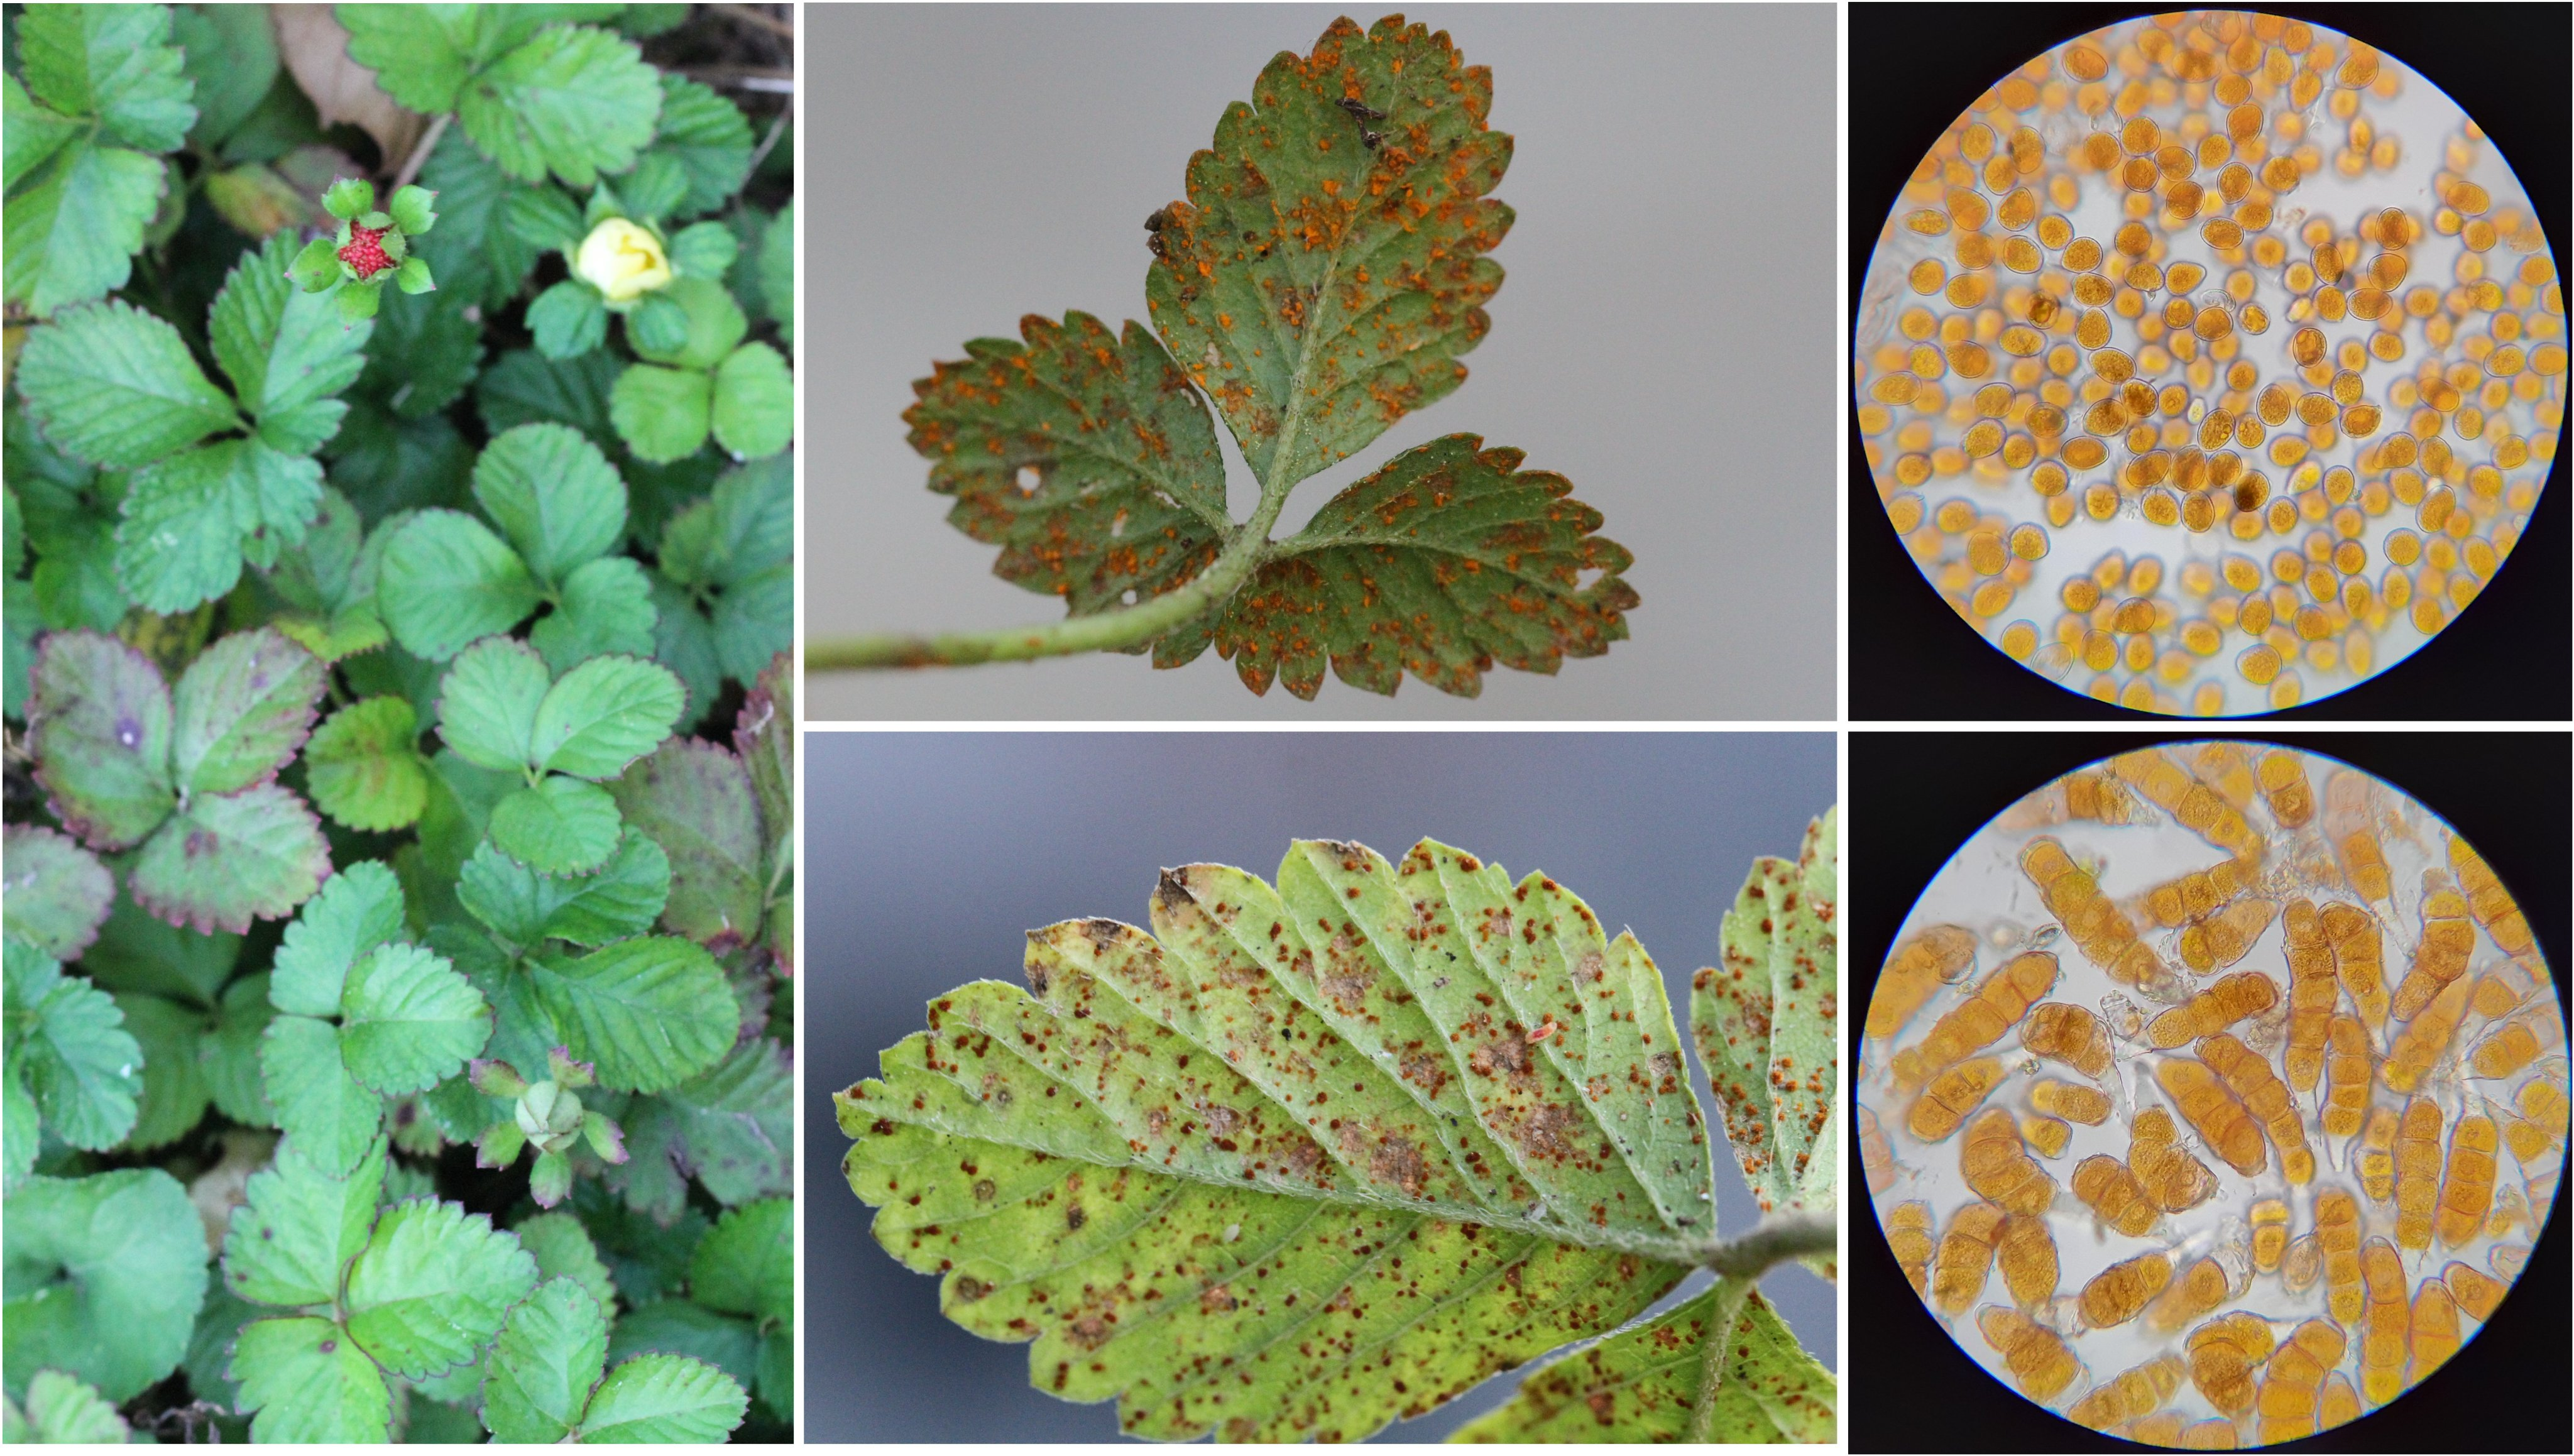
\includegraphics[width=0.92\linewidth]{../images/FCpHrYNWEAIhiv9} \caption{Rust on mock strawberry (\textit{Potentilla indica}) caused by \textit{Phragmidium mexicanum} with urediniospores and teliospores.}\label{fig:strawberry-rust}
\end{figure}

\ecolumns
\end{frame}

\begin{frame}{Causes of plant disease epidemics (The Disease Triangle)}
\protect\hypertarget{causes-of-plant-disease-epidemics-the-disease-triangle}{}
\begin{figure}
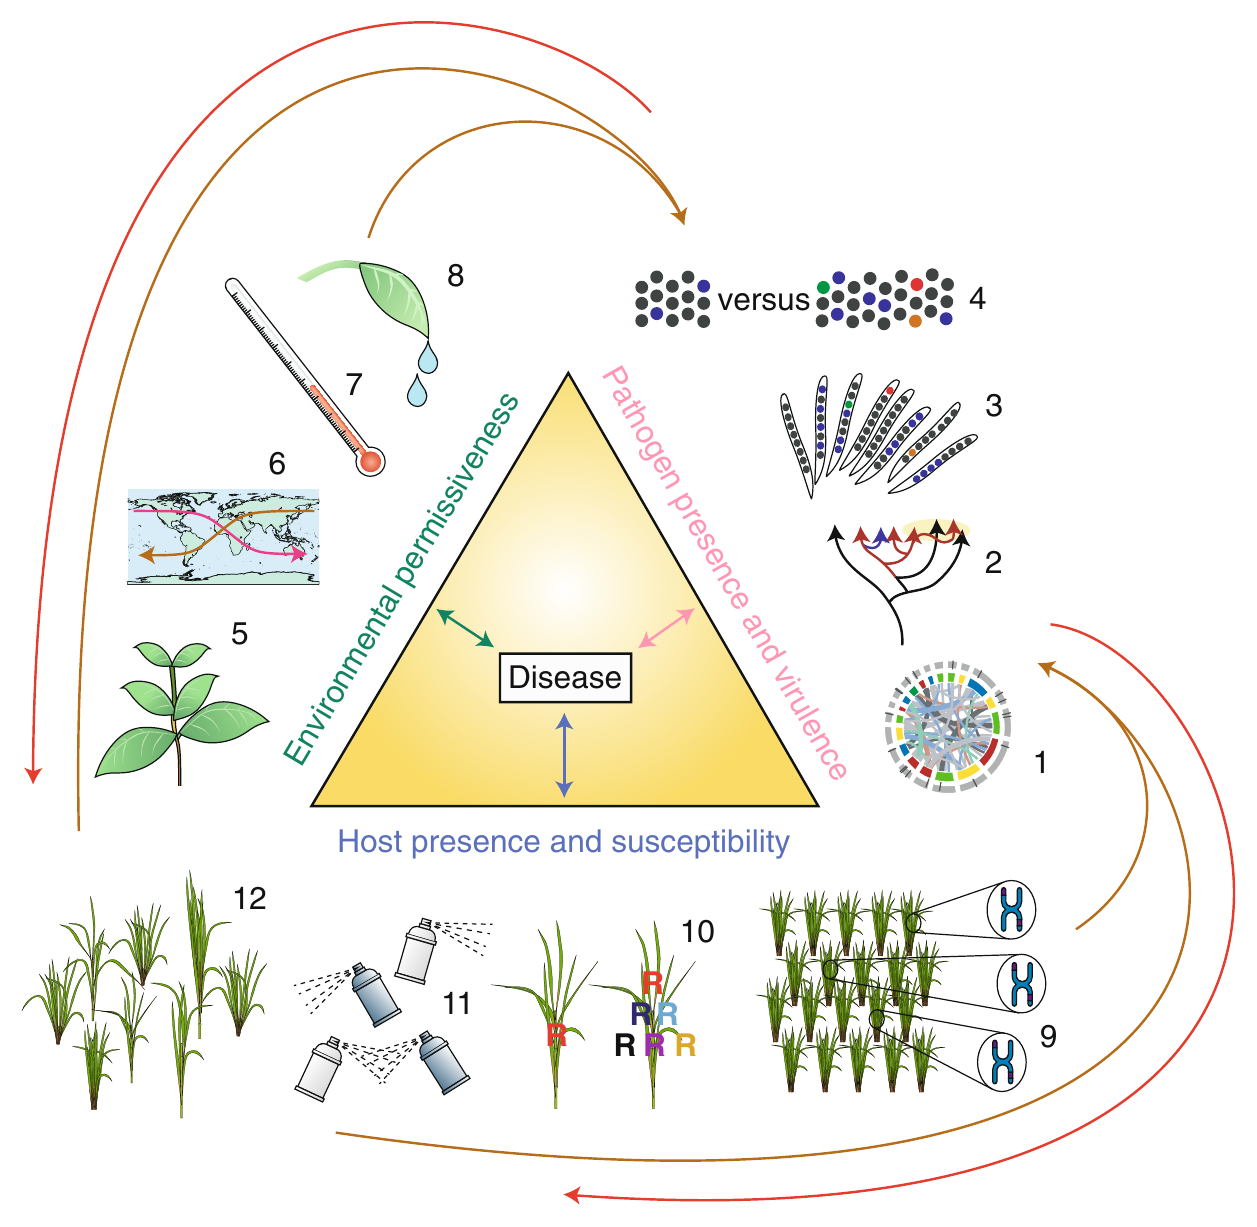
\includegraphics[width=0.45\linewidth]{../images/disease_triangle} \caption{The disease triangle.}\label{fig:disease-triangle}
\end{figure}
\end{frame}

\begin{frame}{}
\protect\hypertarget{section-6}{}
\begin{itemize}
\tightlist
\item
  Infectious disease result from infection caused by plant pathogen.
\item
  Pathogen can grow and multiply rapidly on diseased plants, and can
  spread from diseased to healthy plants and cause additional plant to
  become diseased -- epidemic.
\item
  A plant parasite is an organism that becomes intimately associated
  with a plant and multiplies or grows at the expense of the plant
  (removes nutrients and water from the host)
\item
  Parasitism is associated with pathogenicity, i.e., the ability of a
  pathogen to cause disease, as the ability of the parasite to invade
  and become established in the host generally results in the
  development of a diseased condition.
\end{itemize}
\end{frame}

\begin{frame}{}
\protect\hypertarget{section-7}{}
\begin{itemize}
\tightlist
\item
  Only a few members of a few groups of living organisms can parasitize
  plants.
\item
  Some parasites are biotrophs (obligate parasites, can grow and
  reproduce in nature only in living hosts)

  \begin{itemize}
  \tightlist
  \item
    viruses
  \item
    viroids
  \item
    mollicutes
  \item
    fastidious bacteria
  \item
    nematodes
  \item
    protozoa
  \item
    downy mildew, powdery mildew and rust fungi
  \end{itemize}
\item
  Others are semi-biotrophs (facultative saprophytes), necrotrophs
\item
  Obligate and nonobligate parasites generally differ in the ways in
  which they attack their host plants and procure their nutrients from
  the host
\end{itemize}
\end{frame}

\begin{frame}{Abundance and susceptibility of the host}
\protect\hypertarget{abundance-and-susceptibility-of-the-host}{}
\small

\begin{itemize}
\tightlist
\item
  For most plant disease (particularly foliar) caused by fungi,
  \(\big\Uparrow\) host density \(\sim\) disease \(\big\Uparrow\)
  epidemics.
\item
  \(\big\Uparrow\) the pathogen spores travel from infected source
  plants, \(\big\Downarrow\) concentrated will be the innoculum load
  that reaches the nearest uninfected plants.
\item
  \(\big\Uparrow\) canopy density \(~\) \(\big\Uparrow\) humidity, the
  condition conducive for initial stages of infection.
\item
  Factors contributing to the loss of crop production stability relate
  to:

  \begin{itemize}
  \tightlist
  \item
    \(\big\Uparrow\) field aggregation and size
  \item
    \(\big\Uparrow\) host plant density (\(\big\Uparrow\) fertilizer
    use)
  \item
    \(\big\Uparrow\) crop species uniformity through specialization
  \item
    \(\big\Uparrow\) of genetic uniformity at the cultivar level
  \item
    \(\big\Uparrow\) reliance on race-specific resistance and neglect of
    resistance to currently less-damaging disease
  \end{itemize}
\item
  \(\big\Uparrow\) international exchange of seed and planting stock has
  contributed to the dispersal of pathogens into newer parts of world
\item
  Shorter crop duration \(\big\Uparrow\) pathogen innoculum survival
  from one crop cycle to the next.
\end{itemize}
\end{frame}

\begin{frame}{Environmental factors}
\protect\hypertarget{environmental-factors}{}
\small

\begin{itemize}
\tightlist
\item
  Each pathogen favor a specific set of environmental conditions for
  disease development
\item
  Mostly, soil-borne pathogens are most damaging in wet soil
\item
  Foliar diseases such as wheat stem rust, thrive in hot weather while
  other, such as wheat stripe rust, require cool temperatures.
\item
  Nearly all foliar pathogens (with exclusion of powdery mildew fungi)
  require high moisture for their initial growth on leaf or stem surface
  before they penetrate the interior regions.
\item
  Breeding for disease resistance involves exposing breeding populations
  to induced epidemics or to natural epidemics in known ``hot spots''.
\item
  Breeder's objective is to optimize the pathogen and environmental
  sides of the disease triangle to provide consistent epidemics of
  sufficient severity to clearly damage susceptible breeding lines
  without also destroying lines with useful levels of resistance.
\item
  Three sides of the triangle as main effects as well as interactions
  between them need to be considered.
\end{itemize}
\end{frame}

\begin{frame}{}
\protect\hypertarget{section-8}{}
\begin{itemize}
\tightlist
\item
  Seedling blight in winter wheat is most severe at soil temperatures of
  \SIrange{20}{28}{\celsius} and does not occur below \SI{12}{\celsius}.
\item
  In maize, seedling blight does not occur at soil temperatures above
  \SI{24}{\celsius} and is most severe at \SIrange{8}{20}{\celsius}.
\item
  \(\because\) Wheat, as cool season crop, is adapted to rapid seedling
  development in cool soils, whereas maize is a warm season crop adapted
  to rapid seedling development in warm soils.

  \begin{itemize}
  \tightlist
  \item
    Breeding for reduced seedling blight in early planted maize entails
    selection for lines with greater cold tolerance and faster
    germination in cool soils.
  \end{itemize}
\item
  Susceptibility of upland and lowland ecotypes to rice blast.
\item
  H x E interaction also are prominent in many diseases caused by
  biotrophic pathogens, such as the rust fungi, that are highly
  specialized parasites.
\end{itemize}
\end{frame}

\begin{frame}{}
\protect\hypertarget{section-9}{}
\begin{itemize}
\tightlist
\item
  Pathogen x Environment interactions are encountered in field plot
  tests as:

  \begin{itemize}
  \tightlist
  \item
    non-uniform distribution of soilborne pathogens due to variable
    moisture regimes at low and high spots of the field and due to
    difference in water-holding capacity
  \item
    vector borne virus may be more prominent at the edges of field (edge
    effect)
  \end{itemize}
\item
  Collections of \textit{H. spontaneum} from hot, dry regions of Israel
  were more susceptible to leaf rust and powdery mildew than were
  collections from other areas of Israel where rust and mildew were more
  prevalent.

  \begin{itemize}
  \tightlist
  \item
    disease resistance tend to be lost from plant populations when there
    is no disease pressure to maintain selection for resistance
  \end{itemize}
\end{itemize}
\end{frame}

\hypertarget{resistance-types}{%
\section{Resistance types}\label{resistance-types}}

\begin{frame}{Aspects relating to breeding strategy}
\protect\hypertarget{aspects-relating-to-breeding-strategy}{}
\begin{itemize}
\tightlist
\item
  Inheritance of disease (monogenic or polygenic)
\item
  Effectiveness (complete or partial)
\item
  Specificity (race specific or general)
\end{itemize}
\end{frame}

\begin{frame}{Inheritance}
\protect\hypertarget{inheritance}{}
\small

\begin{itemize}
\tightlist
\item
  \alert{Monogenic} resistance due to a single major gene. It can be
  recognized with certainty and progeny from a cross can be scored as
  either having or lacking that particular gene.
\item
  May not be completely effective, so major genes do not necessarily
  render plants immune from infection.
\item
  In cereal rust diseases several Infection Types (IT) are regarded as
  resistant reaction

  \begin{itemize}
  \tightlist
  \item
    (IT0) reaction show no macroscopic evidence of pathogen attack
    (immunity)
  \item
    (IT;) reaction designated as fleck do not allow pathogen sporulation
    but do show visible evidence of pathogen-induced death of host
    tissue
  \item
    (IT1) reaction is conditioned by genes when very small pustules
    surrounded by a ring of necrotic tissue appear
  \item
    (IT2) reaction is characterized by moderately small pustules
    surrounded by chlorotic halo
  \end{itemize}
\item
  Lr34 gene for leaf rust resistance in wheat only manifests with
  moderate level of adult plant resistance, and is characterized by
  smaller pustules with less sporulation than on fully susceptible
  plants -- hence not a gene for complete resistance.
\end{itemize}
\end{frame}

\begin{frame}{Effectiveness and specificity}
\protect\hypertarget{effectiveness-and-specificity}{}
\small

\begin{itemize}
\tightlist
\item
  Some cultivars with accumulation of many genes for partial resistance
  may remain almost completely free of disease under conditions in which
  fully susceptible cultivars are heavily infected.
\item
  For practical purposes, such form of partial resistance may be said to
  show nearly complete resistance, even if it has no genes for complete
  resistance.
\item
  Race specific versus non-specific resistance addresses the central
  issue of durability of disease resistance in crops.
\item
  \citet{vanderplank2012disease} divided resistance into 2 types (in
  epidemiological terms):

  \begin{itemize}
  \tightlist
  \item
    Vertical (race specific)
  \item
    Horizontal (race non-specific)
  \end{itemize}
\item
  Vertical resistance reduces initial inoculum in an epidemic by
  screening out avirulent races in the pathogen population but has no
  effect on the rate of increase of the virulent races in the epidemic.
\item
  Horizontal resistance reduces the rate of pathogen increase by being
  at least partially effective against all races.
\end{itemize}
\end{frame}

\begin{frame}{}
\protect\hypertarget{section-10}{}
\small

\begin{itemize}
\tightlist
\item
  \citet{simonds1985plant} expanded the classification of resistance
  into 4 types:

  \begin{enumerate}
  \footnotesize
  \item Vertical resistance as defined by Vanderplank,
  \item Pathogen non-specific major gene resistance to cover those cases of monogenic resistance that are known to lack race specificity,
    \begin{itemize}
    \scriptsize
    \item Resistance in maize to \textit{Cochliobolus heterostrophus} due to single gene (a gene for sensitivity of the host to patho-toxin). Pathogens lacking the ability to produce the toxin are avirulent and host plants without the gene for toxin sensitivity are resistant. No alternative form of the toxin gene (HC-toxin) has been found that is not inactivated by the host gene product.
    \item In cultivars of cabbage, single genes for resistance to cabbage yellow disease caused by soilborne \textit{Fusarium oxysporum} f. \textit{conglutinans} haven proven durable.
    \end{itemize}
  \item Horizontal polygenic resistance,
  \item Interaction resistance, which relies on use of mixed populations of host lines with different genes for vertical resistance to avoid rapid selection of races virulent to any single resistance gene in mixture.
  \end{enumerate}
\item
  Induced resistance, even if its effects are only local, may
  substantially reduce the ability of virulent races to infect the
  \alert{same} plants.
\item
  Simmonds suggested that most plants have some level of horizontal
  polygenic resistance against most, if not all, of their diseases.
\end{itemize}
\end{frame}

\begin{frame}{Qualitative and quantitative resistance}
\protect\hypertarget{qualitative-and-quantitative-resistance}{}
\footnotesize

\begin{itemize}
\tightlist
\item
  Terms are used to distinguish both the phenotypic expression of
  resistance and the type of inheritance associated.
\item
  Resistance genes (\(R\)-genes) underlying qualitative resistance tend
  to provide complete or near-complete resistance.
\item
  Studies on major genes have provided understanding of pathogen
  recognition and response.
\item
  \(R\) genes typically show dominant phenotypes and mostly encode
  proteins involved in pathogen recognition.
\item
  Recessive resistance may be caused by loss-of-function variants of
  susceptibility conferring genes (\(S\)-genes)
\item
  Quantitative disease resistance (QDR) shows incomplete or partial
  phenotype and is controlled by multiple genes of small effects.

  \begin{itemize}
  \tightlist
  \item
    helps characterize genetic architecture of resistance in different
    pathosystems
  \end{itemize}
\item
  A cross between a line with strong QDR and one with weak QDR typically
  shows a continuum of phenotypic variation.
\item
  Recent studes on genes conditioning QDR have shown that genes
  resembling R-genes can have incomplete effects and can be identified
  as QTLs in mapping studies.
\item
  Concepts of qualitative and quantitative resistance may not be
  dichotomous, afterall.
\end{itemize}
\end{frame}

\begin{frame}{}
\protect\hypertarget{section-11}{}
\begin{itemize}
\tightlist
\item
  Studies of plant immunity in model systems ( \emph{Arabidopsis
  thaliana}, tomato and rice) have revealed 2 main mechanisms for immune
  response:

  \begin{itemize}
  \tightlist
  \item
    Pathogen-associated molecular pattern (PAMP)-triggered immunity
    (PTI) known as basal resistance -- contributes to quantitative
    resistance
  \item
    Effector-triggered immunity (ETI) -- forms basis of qualitative
    resistance
  \end{itemize}
\item
  PTI is broad-spectrum resistance triggered in response to conserved
  pathogen features as recognized at plant cell surface via conserved
  pattern receptors (PRRs), which are typically membrane-localized
  receptor-like kinases (RLKs) or wall-associated kinases (WAKs).

  \begin{itemize}
  \tightlist
  \item
    PTI is (probably) a component of non-host
    resistance\footnote[frame]{A phenomenon whereby most plants are resistant to most microbial pathogens.}
  \end{itemize}
\end{itemize}
\end{frame}

\begin{frame}{}
\protect\hypertarget{section-12}{}
\bcolumns
\column{0.6\textwidth}

\begin{itemize}
\tightlist
\item
  ETI is activated when R-proteins (encoded by \(R\)-genes) recognize
  their corresponding pathogenic effector protein.
\item
  R-proteins (structural) are typically encoded by nucleotide-binding
  domain leucine-rich repeat containing (NLR) genes, and most R-genes
  encode cytosolic NLR proteins.
\item
  Some R-genes encode detoxification enzymes, while other encode WAKs.
\item
  ETI is often manifested as a hypersensitive response (HR): that is,
  rapid cell death localized at the point of pathogen penetration.
\item
  HR is effective against biotrophic pathogens but increases
  susceptibility to necrotrophic diseases.
\end{itemize}

\column{0.4\textwidth}

\begin{figure}
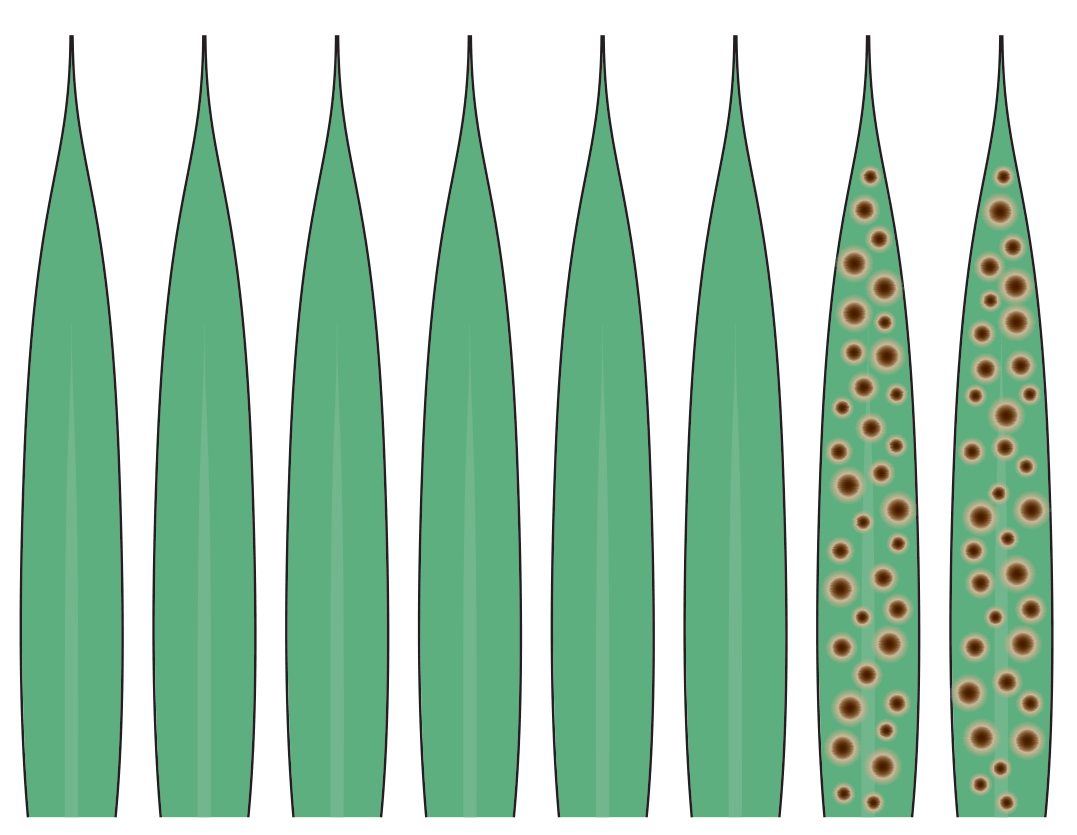
\includegraphics[width=0.55\linewidth]{../images/qualitative_resistance} \caption{Qualitative resistance}\label{fig:qualitative-res}
\end{figure}

\begin{figure}
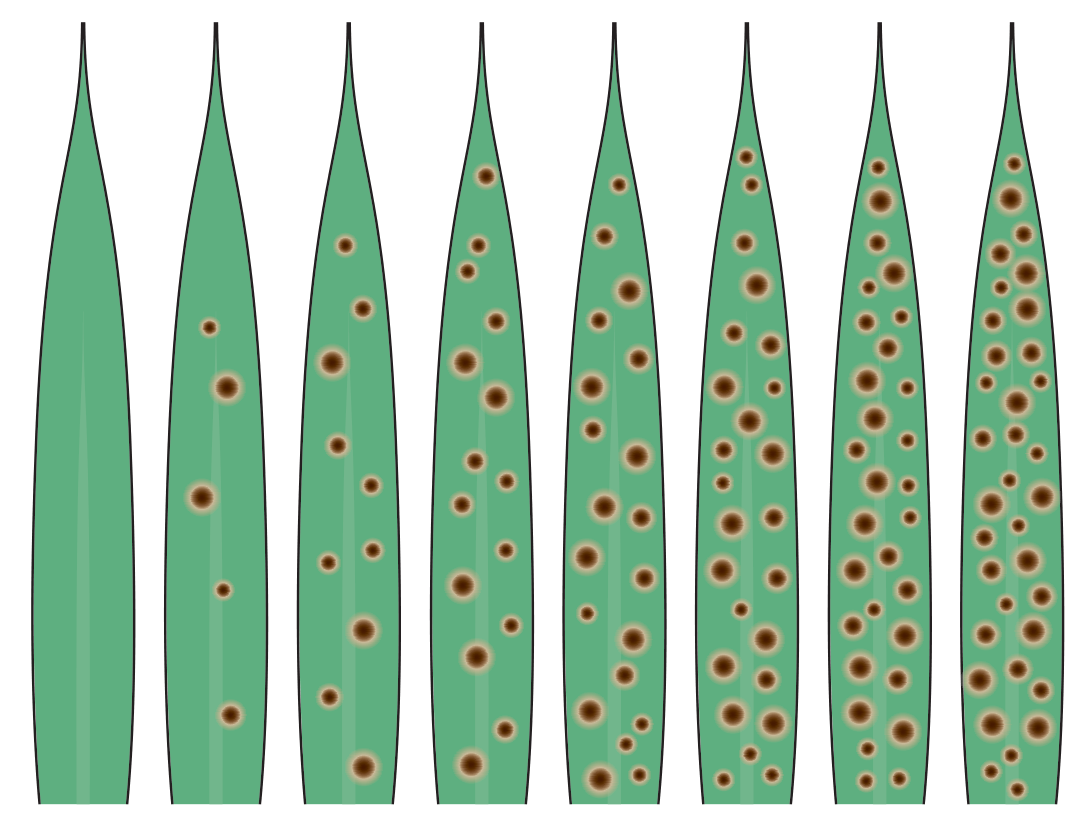
\includegraphics[width=0.55\linewidth]{../images/quantitative_resistance} \caption{Quantitative resistance}\label{fig:quantitative-res}
\end{figure}

\ecolumns
\end{frame}

\begin{frame}{Hypersensitive resistance}
\protect\hypertarget{hypersensitive-resistance}{}
\bcolumns
\column{0.65\textwidth}
\begin{description}
\item[Hypersensitive reaction] Host in which intial contacts in incompatible combinations of avirulent pathogen with resistant host trigger rapid death of the contacted host cells with release of metabolites injurious to the pathogen.
\end{description}

\small

\begin{itemize}
\tightlist
\item
  The challenge with polygenic nonspecific resistance is to recognize
  the resistance as non-specific when it occurs in breeding population.
\item
  Best documented cases of race-specific resistance are based on
  hypersensitive reaction.
\item
  For diseases caused by biotrophic pathogens, hypersensitive resistance
  is generally of race-specific type.
\end{itemize}

\column{0.35\textwidth}

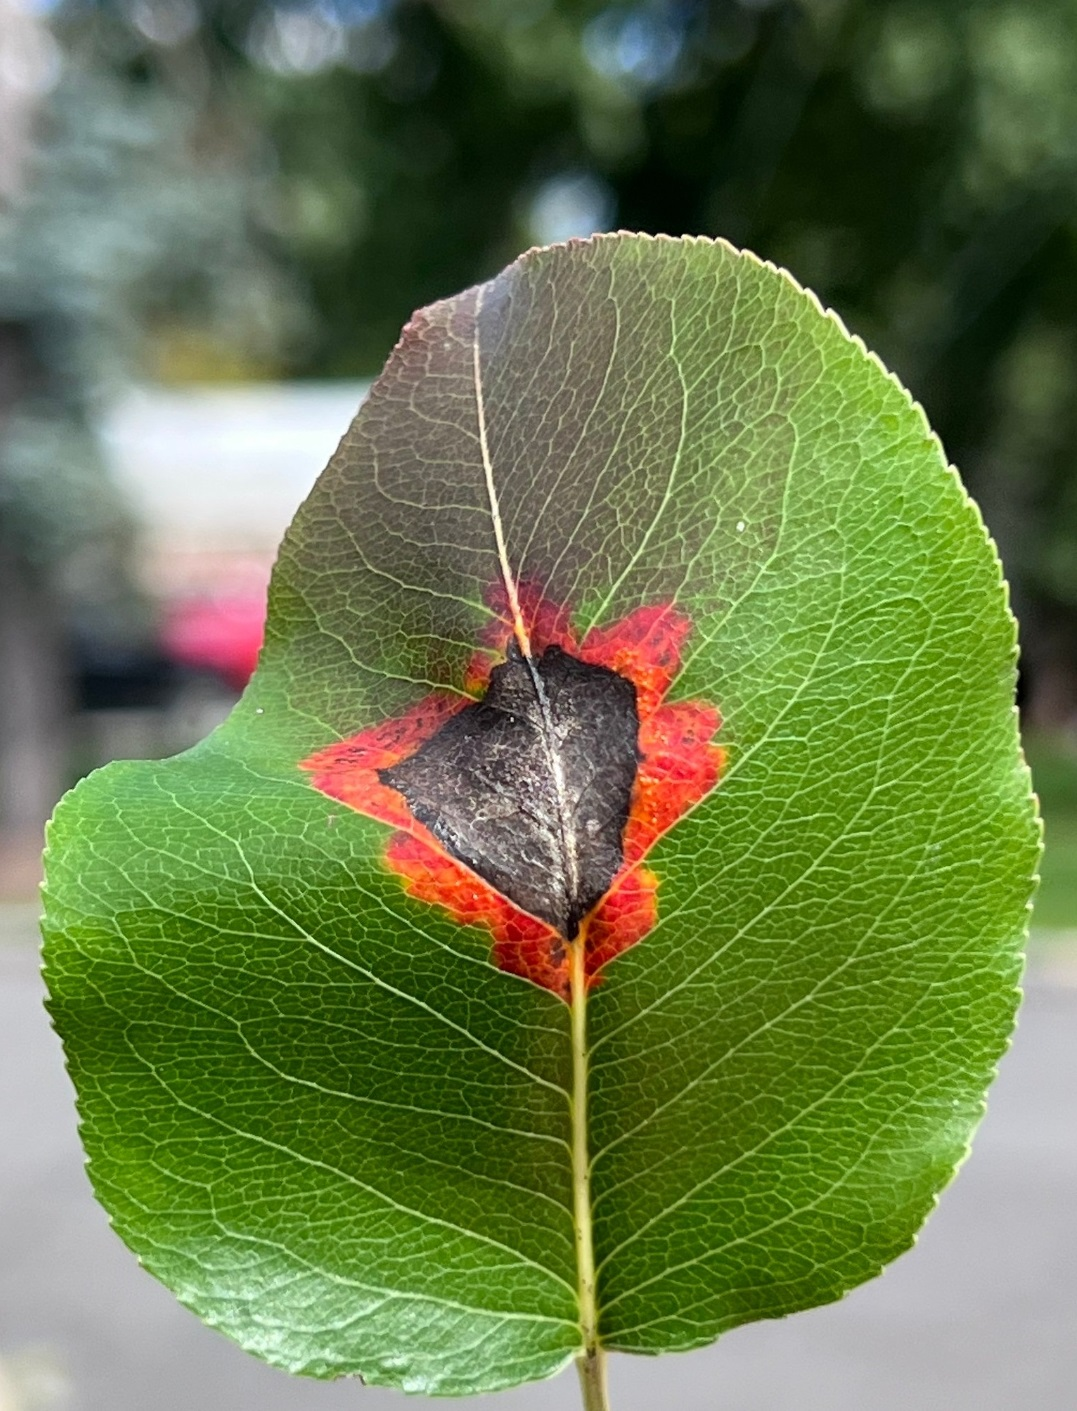
\includegraphics[width=0.7\linewidth]{../images/hypersensitive_reaction}

\ecolumns
\end{frame}

\begin{frame}{}
\protect\hypertarget{section-13}{}
\begin{itemize}
\tightlist
\item
  R-genes have typically been identified by approaches including:

  \begin{itemize}
  \footnotesize
  \item fine-mapping and positional cloning,
  \item mutation screening and \hspace{1.5cm}
  \smash{\raisebox{.25\dimexpr2\baselineskip+1\itemsep+2\parskip}{$\left.\rule{0pt}{.6\dimexpr2\baselineskip+1\itemsep+2\parskip}\right\}$\ \parbox{4cm}{Qualitative resistance}}}
  \item systematic identification and testing of NLR genes (using homology)
  \end{itemize}
\item
  Identification and analysis of R-genes has proceeded more quickly than
  that for genes conditioning minor effects, hence R-cloning is easier
  than QTL cloning.
\item
  One strategy in identification of R-genes that are likely to be
  effective for resistance breeding entails sequencing the existing
  pathogen population to characterize the relevant effectors and then
  deploying R-genes that recognize those effectors.

  \begin{itemize}
  \tightlist
  \item
    using combination of bioinformatic and functional approaches
  \end{itemize}
\item
  R-genes are extremely specific and provide resistance against one or
  few strain/races of a particular pathogen.

  \begin{itemize}
  \footnotesize
  \item R-genes (especially NLR genes) are found in tightly linked clusters
  \item Clustering reflects and allows evolutionary diversification of recognition specificities or R-genes \cite{hulbert2001resistance}
  \end{itemize}
\end{itemize}
\end{frame}

\begin{frame}{}
\protect\hypertarget{section-14}{}
\small

\begin{itemize}
\tightlist
\item
  Most studies on quantitative resistance have focused on the underlying
  genetic architecture, which is relevant for crop improvement rather
  than on the identity and mechanisms of individual genes

  \begin{itemize}
  \tightlist
  \item
    linkage analysis
  \item
    GWAS (better resolution of candidate genes for
    validation\footnote[frame]{Validation of gene entails transformation or mutatgenesis experiments to confirm the presence/absence})
  \end{itemize}
\item
  Mapping studies have shown that resistance is often a polygenic trait
  -- that produces a continuous distribution of phenotypes in a
  biparental cross.
\item
  Mapping studies (synthesized study) for disease have: \bitemize
  \footnotesize

  \item

  Rice \(\longrightarrow\) 16 studies \(\longrightarrow\) 94 QRLs
  \(\longrightarrow\) cover more than half the genome

  \item

  Maize \(\longrightarrow\) 50 studies \(\longrightarrow\) 437 QRLs
  cover 89\% of the genome

  \item

  This is still underestimation of true number of loci \eitemize
\item
  Underlying genetic mechanism for most QRLs is unknown, however,
  \bitemize \footnotesize

  \item

  Many of the genes are similar in sequence to NLR genes, PRR genes or
  defence genes that can be controlled by these recognition-related
  genes

  \item

  In some cases, multiple linked genes (such as groups of functionally
  related defence genes involved in secretory process and cell wall
  reinforcement) have been shown to underlie a single QRL \eitemize
\end{itemize}
\end{frame}

\begin{frame}{}
\protect\hypertarget{section-15}{}
\begin{figure}
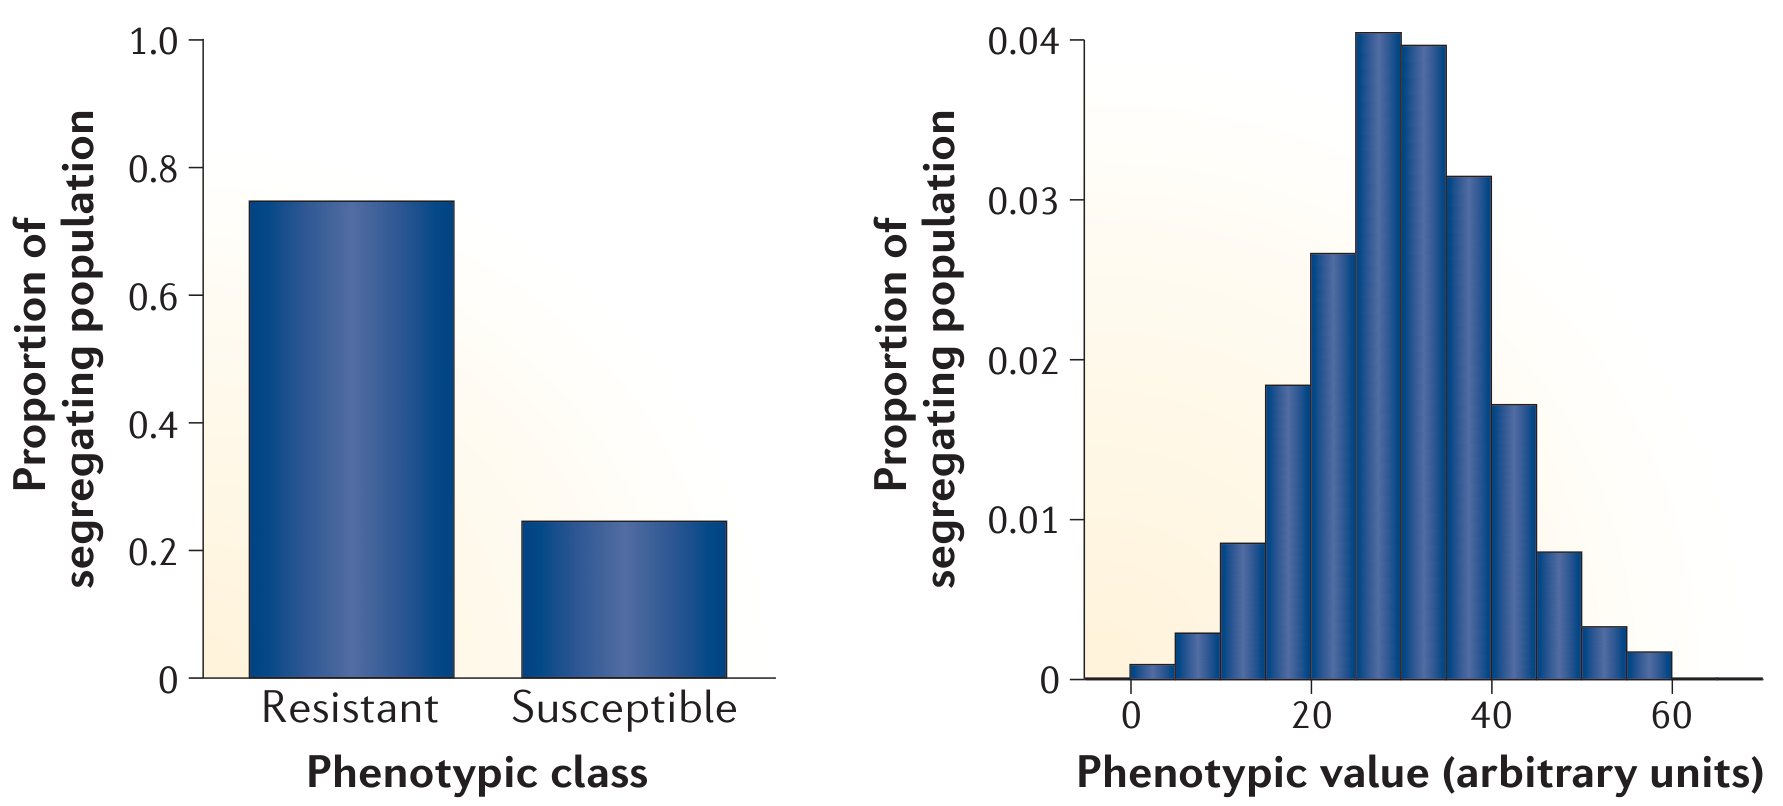
\includegraphics[width=0.99\linewidth]{../images/qualitative_quantitative_segregation} \caption{In a segregating population, a dominant major gene conditioning qualitative resistance segregates in a 3:1 ratio, while multiple genes of small effect contribute to continuous phenotypic variation for quantitative resistance.}\label{fig:quantitative-qualitative-segregation}
\end{figure}
\end{frame}

\begin{frame}{}
\protect\hypertarget{section-16}{}
\begin{figure}
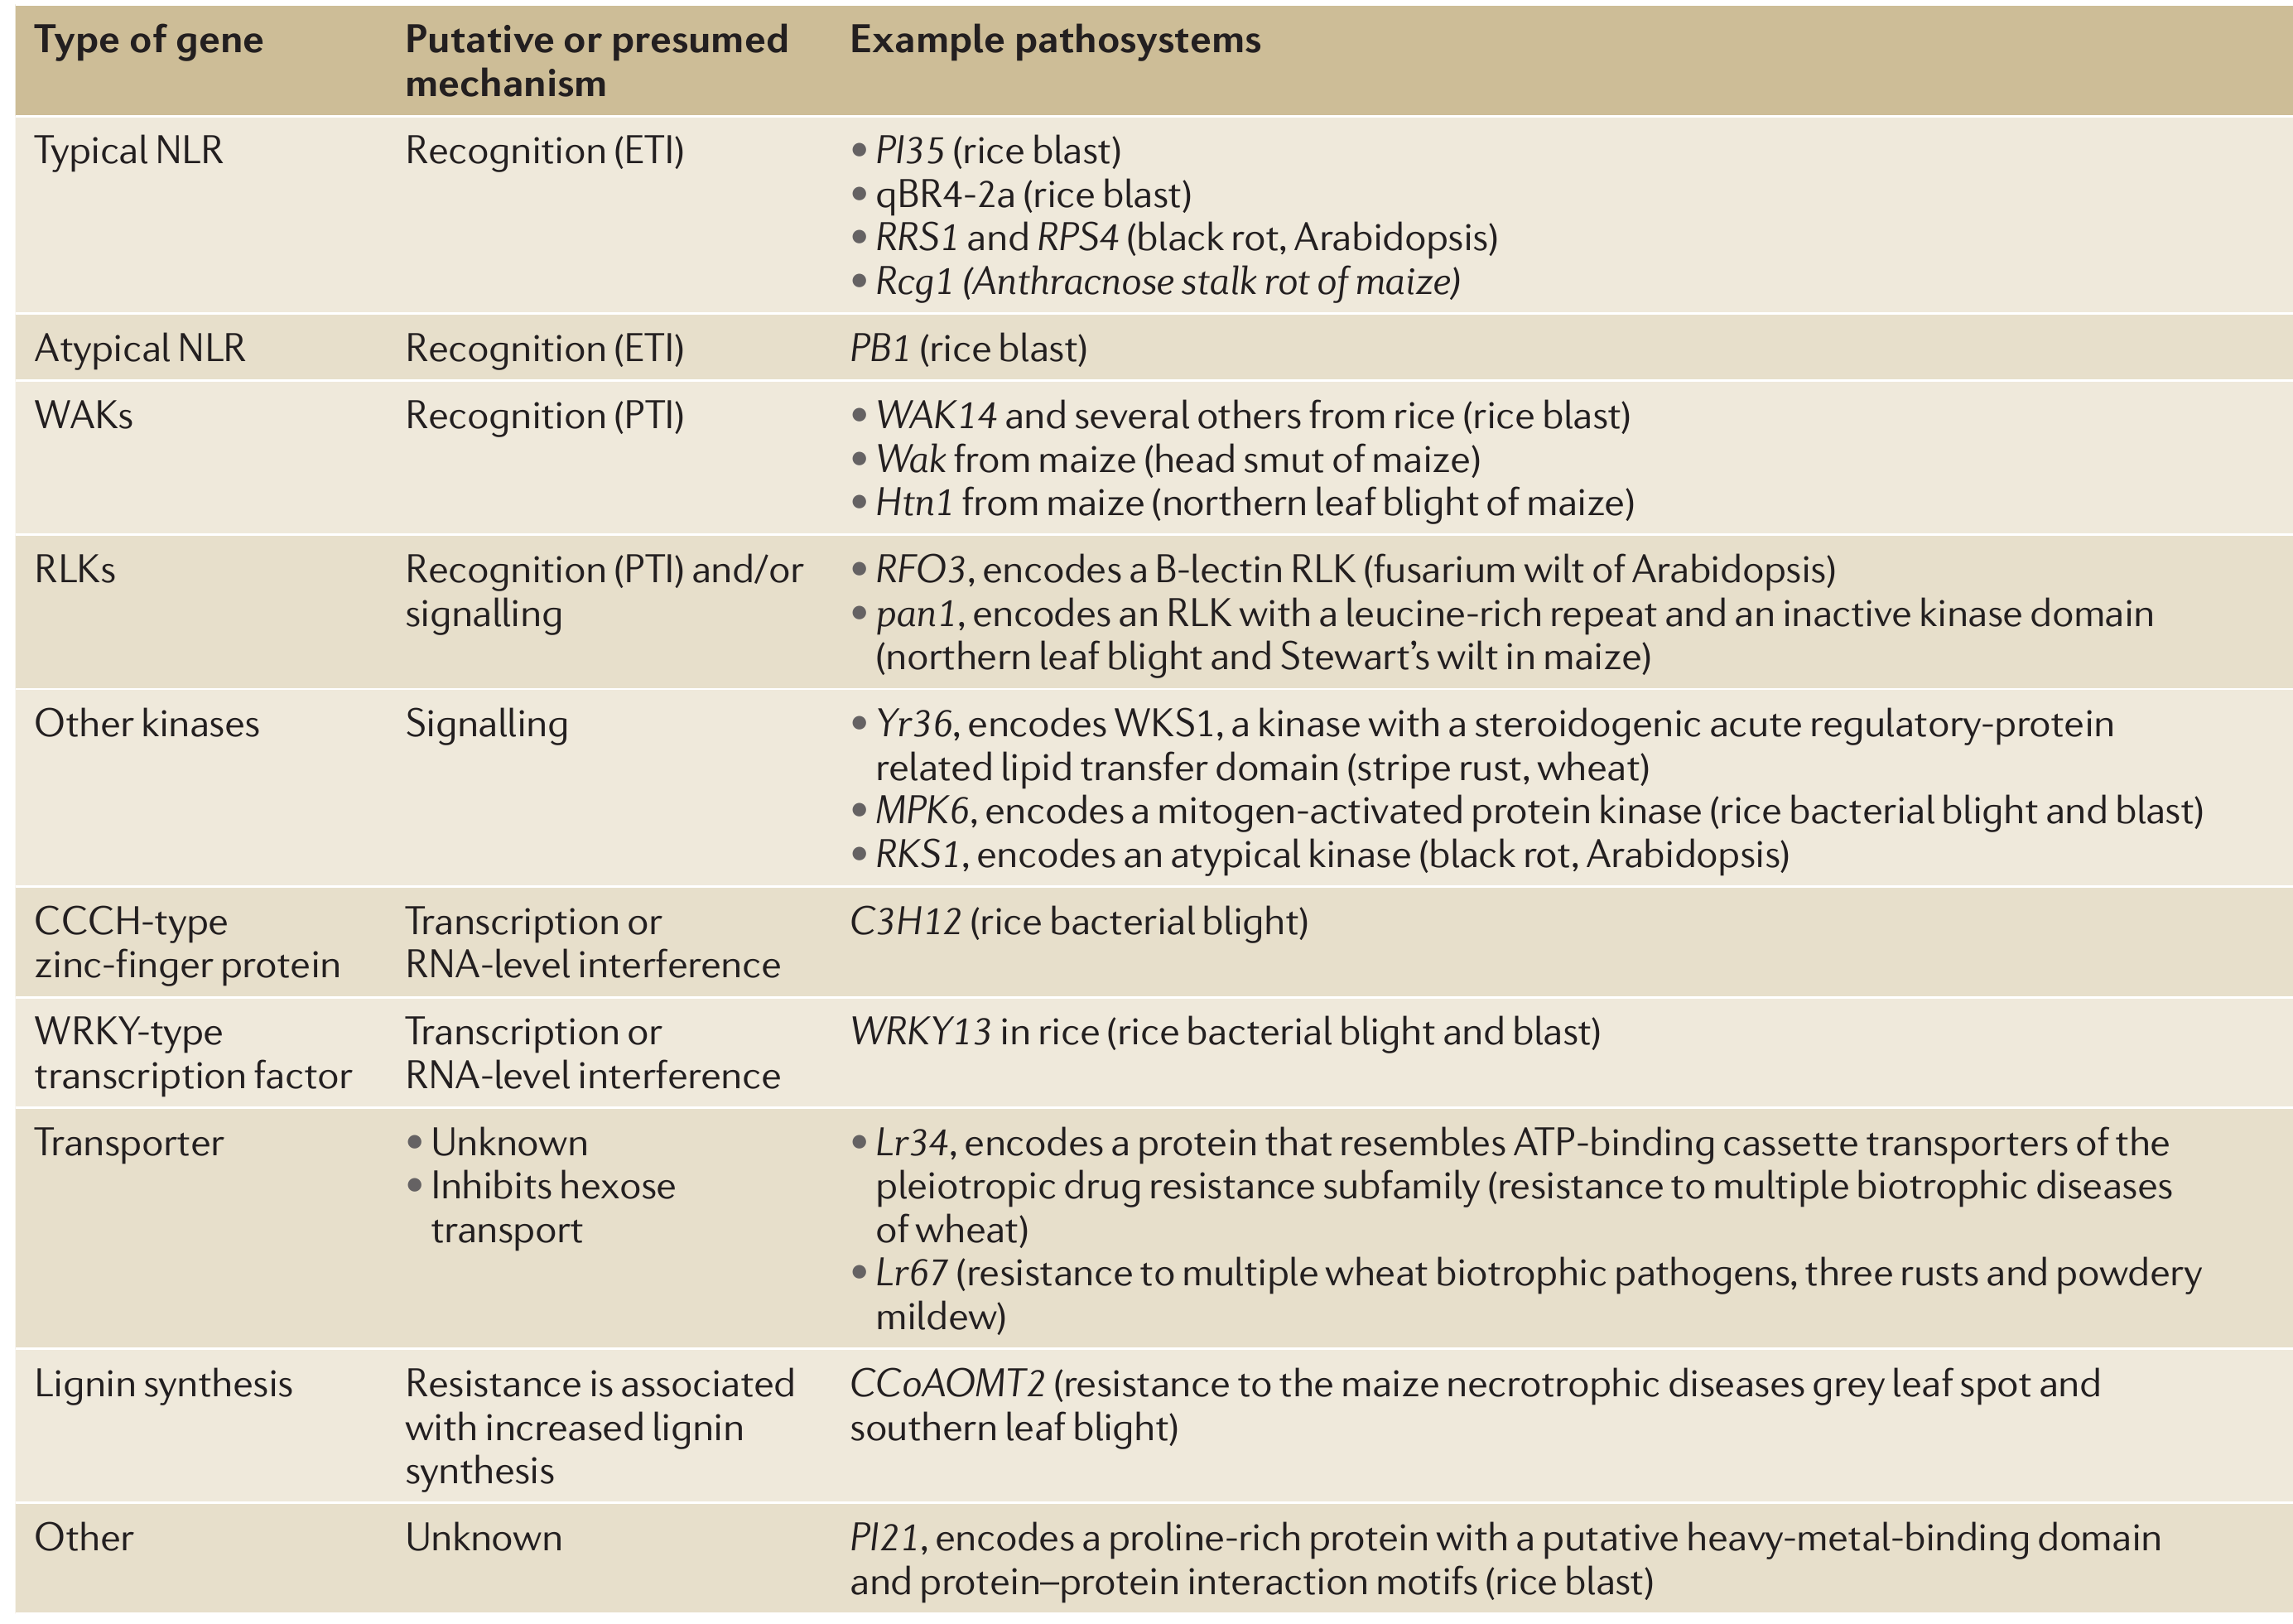
\includegraphics[width=0.7\linewidth]{../images/quantitative_candidate} \caption{Example of different types of causal and candidate genes that contribute to quantitative resistance. \cite{nelson2018navigating}.}\label{fig:quantitative-candidate-genes}
\end{figure}
\end{frame}

\hypertarget{disease-resistance-mechanisms}{%
\section{Disease resistance
mechanisms}\label{disease-resistance-mechanisms}}

\begin{frame}{Disease escape or avoidance}
\protect\hypertarget{disease-escape-or-avoidance}{}
\begin{itemize}
\tightlist
\item
  May not even a true resistance mechanism

  \begin{itemize}
  \tightlist
  \item
    maturing plants may complete their growth and produce seeds before
    epidemics of foliar diseases have progressed far enough to cause
    significant damage
  \end{itemize}
\item
  Wheat stem rust epidemics in US begin with overwintered infections in
  winter wheat plants near the Gulf Coast. \textit{P. graminis} develops
  best in warm weather, so stem rust epidemics develop slowly during the
  spring. One reason for the decline of stem rust damage in the Central
  Plains states of Oklahoma and Kansas was the switch to earlier
  maturing winter wheat cultivars in those states in the 1930s and
  1940s.
\item
  Reduction in the population density of host plants
\end{itemize}
\end{frame}

\begin{frame}{Morphological resistance}
\protect\hypertarget{morphological-resistance}{}
\begin{itemize}
\tightlist
\item
  Morphological feature of plants enabling them to avoid infection
\item
  Tuber rot in stored potatoes is initiated primarily in wounds to the
  tubers incurred during harvesting/transport. Rapid healing by
  development of a suberized layer over the wounded tissue is considered
  most critical aspect of resistance therein.
\item
  Floral development is important in the resistance of wheat to ergot
  caused by \textit{Claviceps purpurea}.

  \begin{itemize}
  \tightlist
  \item
    pathogen invades the ovules by way of stigmas of the rye florets
  \item
    \(\because\) rye is typically cross-pollinated, the unfertilized
    stigmas are exposed to ascospores
  \item
    however, once ovules are fertilized, stigmas are no longer receptive
    to infection
  \item
    \(\because\) wheat is self-pollinated, stigmas are no longer
    receptive to infection by the time they become exposed to pathogen
    spores in air
  \item
    male sterile lines of wheat tend to be infected heavily as rye by
    ergot!
  \end{itemize}
\end{itemize}
\end{frame}

\begin{frame}{}
\protect\hypertarget{section-17}{}
\begin{itemize}
\tightlist
\item
  Failure of anther extrusion in barley cultivars leads to partial
  escape from Fusarium head blight.
\item
  Covering of leaf epidermis with hairs or waxes that repel water
\item
  Upright geometry of foliage cause water droplets to roll off the
  leaves allowing them to dry rapidly
\item
  Plants unattractive to potential vectors escape infection even if they
  are susceptible to the vector-borne pathogen
\item
  Rice cultivars selected for more efficient silicon uptake have
  morphological resistance to \textit{M. grisea} (mentioned earlier).
\item
  In wheat stem rust caused by \textit{P. graminis}:

  \begin{itemize}
  \tightlist
  \item
    seedlings exhibit no morphological resistance
  \item
    adult plants allow growth of pathogen only in the chlorophyllous
    collenchyma bundles of stems
  \item
    cultivars with narrow, isolated strands of collenchyma bundles
    separated by broad bands of sclerenchyma are partially resistant to
    stem rust in adult plants
  \end{itemize}
\end{itemize}
\end{frame}

\begin{frame}{Chemical barrier to invasion}
\protect\hypertarget{chemical-barrier-to-invasion}{}
\begin{itemize}
\tightlist
\item
  Chemical defense compounds with general antibiotic properties:

  \begin{itemize}
  \tightlist
  \item
    tannins
  \item
    phenolic compounds
  \item
    dienes
  \item
    saponins
  \item
    proteases
  \item
    hydrolytic enzymes
  \end{itemize}
\item
  Seeds typically have higer concentration of antibiotic compounds than
  vegetaive parts of annual plants
\end{itemize}
\end{frame}

\begin{frame}{Induced response to invasion}
\protect\hypertarget{induced-response-to-invasion}{}
\footnotesize

\begin{itemize}
\tightlist
\item
  Plants respond to woulds in a non-specific production of corky tissue
  that wall off the broken area of the epidermis. Similar barriers are
  produced in the woody stems and roots of trees or other perennial
  plants in response to canker-forming pathogens.

  \begin{itemize}
  \tightlist
  \item
    speed at which a plant produces such barrier is a measure of its
    generalized resistance
  \end{itemize}
\item
  Cell walls in the epidermis may induce thickenings in reponse to
  pathogens attempting to penetrate their outer walls.

  \begin{itemize}
  \tightlist
  \item
    walls thickenings are often infused with phenolic substances
  \end{itemize}
\item
  Wilt disease fungi typically grow through the xylem and tend to cut
  off water flow to aerial parts of the plant

  \begin{itemize}
  \tightlist
  \item
    plant may wall off the pathogen by forming tyloses within xylem
    cells
  \end{itemize}
\item
  Plants activate pathways to produce characteristic antibiotic
  compounds called phytoalexins in the cells around the site of attack

  \begin{itemize}
  \tightlist
  \item
    if the response is soon enough and extensive, plant may display
    partial resistance
  \end{itemize}
\item
  The rate of response of the host may depend on its ability to
  recognize that it is being invaded.
\end{itemize}
\end{frame}

\hypertarget{genome-comparisons-of-plant-pathogens-filamentous}{%
\section{Genome comparisons of plant pathogens
(filamentous)}\label{genome-comparisons-of-plant-pathogens-filamentous}}

\begin{frame}{}
\protect\hypertarget{section-18}{}
\begin{figure}
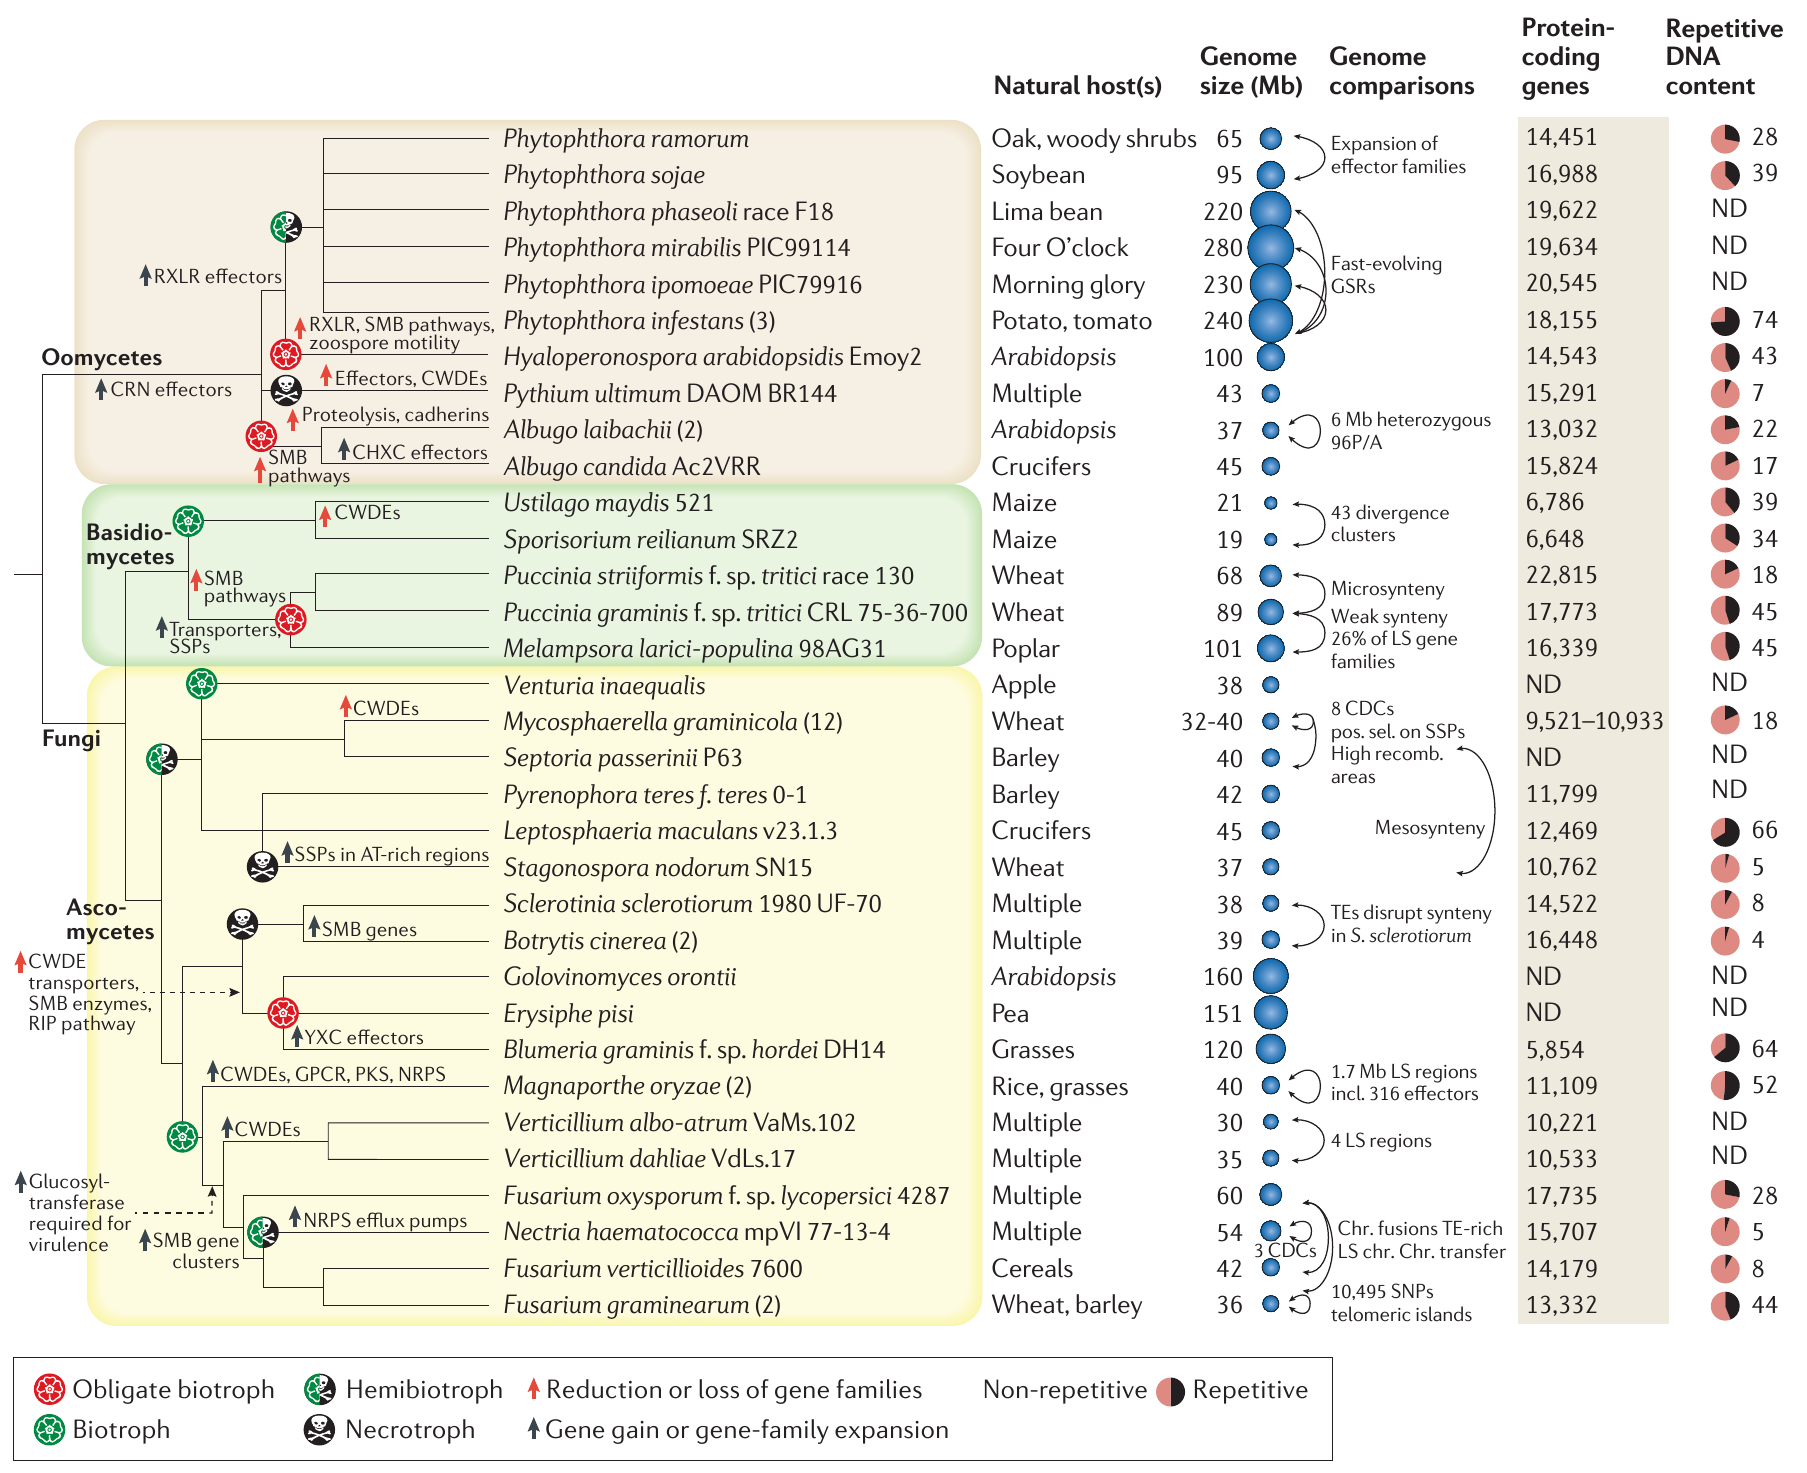
\includegraphics[width=0.4\linewidth]{../images/genome_comparison_pathogenic_fungi} \caption{Main features of sequenced filamentous plant pathogen genomes. Filamentous eukaryotic plant pathogens belong to either the fungi or the stramenopiles (oomycetes). The representative phylogeny depicts filamentous plant pathogens with sequenced genomes and has been generated using iTOL with NCBI taxonomy identifiers (branch lengths are arbitrary). Isolate identifier, or the number of isolates sequenced, is indicated next to the species name. Pathogen lifestyles and major variations in gene families are indicated along the tree branches. The principal host plants, genome size, main insights gained from genome comparisons, number of predicted protein-coding genes and repetitive DNA content (as a percentage of genome size) are shown next to the tree branches. CDC, conditionally dispensible chromosome; chr., chromosome; CNV, copy number variation; CRN, Crinkler; CWDE, cell wall-degrading enzyme; GPCR, G protein coupled receptor; GSR, gene-sparse region; incl., including; LS, lineage-specific; ND, not determined; NRPS, non-ribosomal peptide synthetase; P/A, presence/absence; PKS, polyketide synthase; pos. sel., positive selection; rec., recombination; RIP, repeat-induced point; SMB, secondary metabolite biosynthesis; SNPs, single-nucleotide polymorphisms; SSP, small secreted protein; TE, transposable element}\label{fig:pathogenic-fungi-genome-compare}
\end{figure}
\end{frame}

\hypertarget{genetic-fine-structure-of-resistance-loci}{%
\section{Genetic fine structure of resistance
loci}\label{genetic-fine-structure-of-resistance-loci}}

\begin{frame}{}
\protect\hypertarget{section-19}{}
Refer to Chapter 2 of \citet{hulbert1997genetic}.
\end{frame}

\hypertarget{breeding-for-disease-resistance}{%
\section{Breeding for disease
resistance}\label{breeding-for-disease-resistance}}

\begin{frame}{}
\protect\hypertarget{section-20}{}
\small

\begin{itemize}
\tightlist
\item
  To address ever evolving relationship between host-pathogen
  interaction, resistance breeding programmes systematically test wild
  relatives, landraces and other germplasm to identify new genetic
  sources of resistance to important pests and pathogens.
\item
  Simple resistance (based on single gene) can be effective in short
  term, but successful long term resistance requires dealing with
  genetic complexity.
\item
  Effective disease resistance depends on phenomena thay play out at
  level of genes, genotypes and populations.
\item
  Gene and genomic loci conferring resistance can be assessed in terms
  of the strength of their effect, their race specificity and their
  potential contribution towards durability.
\item
  At genotype level, performance of resistance is influenced by the
  number of resistance genes and their specific combination in host

  \begin{itemize}
  \tightlist
  \item
    indirect effects on valued traits also need to be taken into account
  \end{itemize}
\item
  At population level, effects on the durability of resistance and the
  spread of disease need to be considered
\end{itemize}

(\footnotesize Based on a Review article by
\citet{nelson2018navigating})
\end{frame}

\begin{frame}{}
\protect\hypertarget{section-21}{}
\small

\begin{itemize}
\tightlist
\item
  Plant breeders prefer broad-spectrum (race-nonspecific) resistance
  conferred by QRLs.
\item
  Genes conferring multiple disease resistance (MDR) are much valued --
  they tend also to be durable. \bitemize \footnotesize

  \item

  Causal genes for MDR are not clearly identified

  \item

  But, either genetic linkage or pleiotropy have roles in MDR

  \item

  Single pleiotropic gene or tightly linked genes can be moved between
  cultivars through traditional breeding

  \item

  example: \textit{LR34} (encodes an ATP-binding cassette transporter
  rather than an NLR and provides incomplete resistance;
  \alert{it can actually be considered to be a strong QRL}) in wheat
  condition such resistance \eitemize
\item
  Combining multiple R-genes and/or QRLs into a single genome usually
  improves its resistance phenotype -- an approach called gene
  pyramiding.
\end{itemize}

\begin{table}

\caption{\label{tab:diff-qrl-pyramid}Difference between gene pyramid and QRL}
\centering
\fontsize{6}{8}\selectfont
\begin{tabular}[t]{>{\raggedright\arraybackslash}p{24em}>{\raggedright\arraybackslash}p{30em}}
\toprule
QRL & Gene pyramid\\
\midrule
QRL are generally additive in effect, although non-additive effects are also sometimes observed & Pyramiding of R-genes can improve the spectrum of resistance; genes with complementary resistance spectra can be selected such that gene pyramids provide resistance to a broad set of pathogen races\\
\bottomrule
\end{tabular}
\end{table}
\end{frame}

\hypertarget{references}{%
\section{References}\label{references}}

\begin{frame}{References}
\renewcommand{\bibname}{References} 
\scriptsize
\end{frame}

          \begin{frame}[allowframebreaks]{}
    \bibliographytrue
    \bibliography{./../bibliographies.bib}
    \end{frame}
  


\end{document}
